\section{Motion planning}
Motion planning is the problem of finding a sequence of valid actions that will transform the robot from its initial configuration to a desired configuration. Such actions can be constrained: we might ask the robot to avoid obstacles, to respect its kinematic limits, or to minimize energy consumption. 

We will first introduce a mathematical framework to describe the robot's configuration space, obstacles, and collision, then we will present some algorithms to solve the motion planning problem.

\subsection{Configuration space}
\subsubsection{Definitions}
The ambient space, also called the \emph{workspace}, is in most cases the Euclian manifold $\E^3$. In this ambient space, a physical system can be described as a set of compacts subsets called \emph{bodies}. The vector of the considered physical systems must be in the \emph{state space} $\S$, the set of all possible sets:
\begin{equation*}
    (K_1, \dots, K_N) \in\S \subseteq \mathcal{K}(\E^3)^N
\end{equation*}

The state space is parametrized with a transformation $q$ in the \emph{configuration space} $\Cc$:
\begin{equation*}
    q = (\varphi_1, \dots, \varphi_M)\in\Cc
\end{equation*}
where each $\varphi_i$ is a \emph{transformation} of a system, that is:
\begin{equation*}
    \varphi_i: \mathcal{K}(\E^3) \to \mathcal{K}(\E^3)
\end{equation*}
Note that $M$ corresponds to the number of systems of the robot, the other physical systems being obstacles. Therefore, given a configuration $q$, the space $S_q$ is:
\begin{equation*}
    S_q = \underbrace{\varphi_1(K_1^\circ), \dots, \varphi(K_M^\circ)}_{\text{robot}}, \underbrace{K_{M+1}, \dots, K_N}_{\text{obstacles}}
\end{equation*}
where the $K_i^\circ$ are compacts representing each body, intuitively in their own frames. We will see below that they can be represented numerically with meshes or polynomials.

In general, $\Cc$ is a manifold, its dimension being the number of degrees of freedom of the system. Note that the numerical dimension used to represent $\Cc$ is not necessarily the same as the actual dimension of the manifold: for instance, quaternions of dimension 4 can be used to represent rotations of $SO(3)$, a manifold of dimension 3.

\subsubsection{Joints}
Multiple types of joints can be used to connect the different parts of a robot. Formally, a joint is a mapping from a manifold of dimension $1\leq p\leq6$ into the solid placement $SE(3)$. The difference between the joints is the dimension of the manifold, which can also be seens as the number of degrees of freedom of the joint.
\begin{figure}
    \centering
    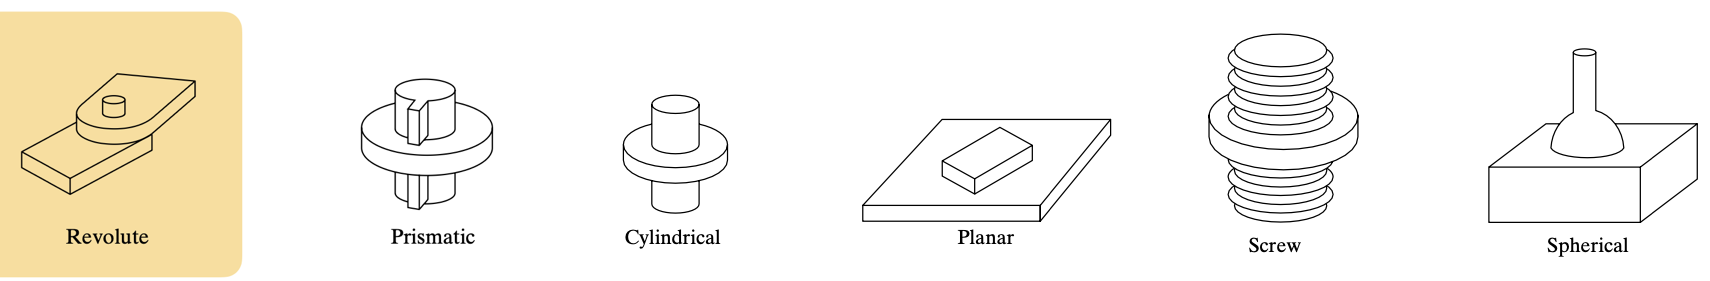
\includegraphics[width=.7\textwidth]{motion-planning/joints.png}
    \caption{Different types of joints.}
\end{figure}

\subsubsection{Examples}
\paragraph*{Moving solid}
Let us consider the Euclidian manifold $\E^2$ as a workspace, that is 2D objects. A solid object $K$ is described as a compact subset of $\E^2$. The configuration space is the set of transformations of this object, $SE(2)$, the special Euclidian group of dimension 2.

\paragraph*{Double pendulum}
In the case of a double pendulum, the workspace remains $\E^2$. Because of the physical constraints on the structure of the system, the pendulum is parametrized by two angles $\theta_1$ and $\theta_2$. The configuration space is therefore a torus $T^2=S^1\times S^1$, but can also be seen as $[0,2\pi)\times[0,2\pi)$.

\paragraph*{Rigid poly-articulated body}
The same general framework can be applied to more complex systems, such as humanoid robots. The workspace is $\E^3$, and the configuration $q$ of a robot is represented by the concatenation of the parameters of each joint:
\begin{equation*}
    q\in \underbrace{SE(3)}_{\text{Position}} \times \underbrace{S_1\times \dots\times S_1}_{\text{Revolute joints}} \times \underbrace{[0,1]\times\dots\times[0,1]}_{\text{Prismatic \& bounded joints}}
\end{equation*}
Recall that the forward kinematic can be used to compute the position of each joint in the global frame, given the configuration $q$.

\begin{figure}[H]
    \centering

    \begin{minipage}{0.4\textwidth}
        \centering
        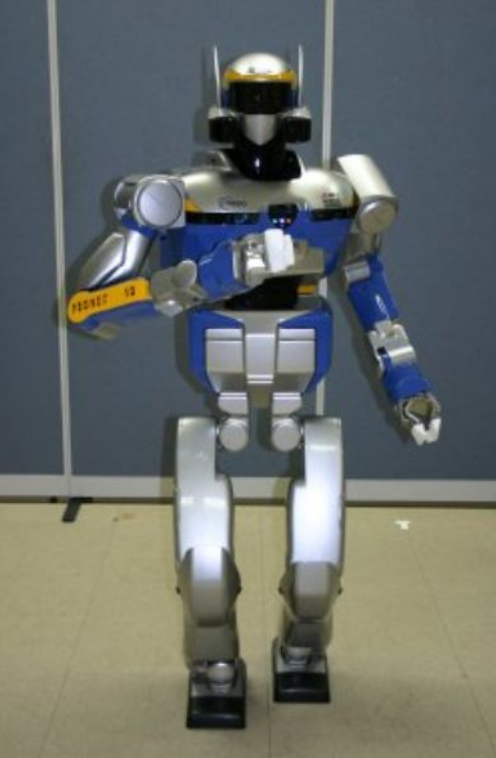
\includegraphics[width=.5\textwidth]{motion-planning/humanoid.png}
        \caption*{A humanoid robot}
    \end{minipage}
    \begin{minipage}{0.5\textwidth}
        \centering
        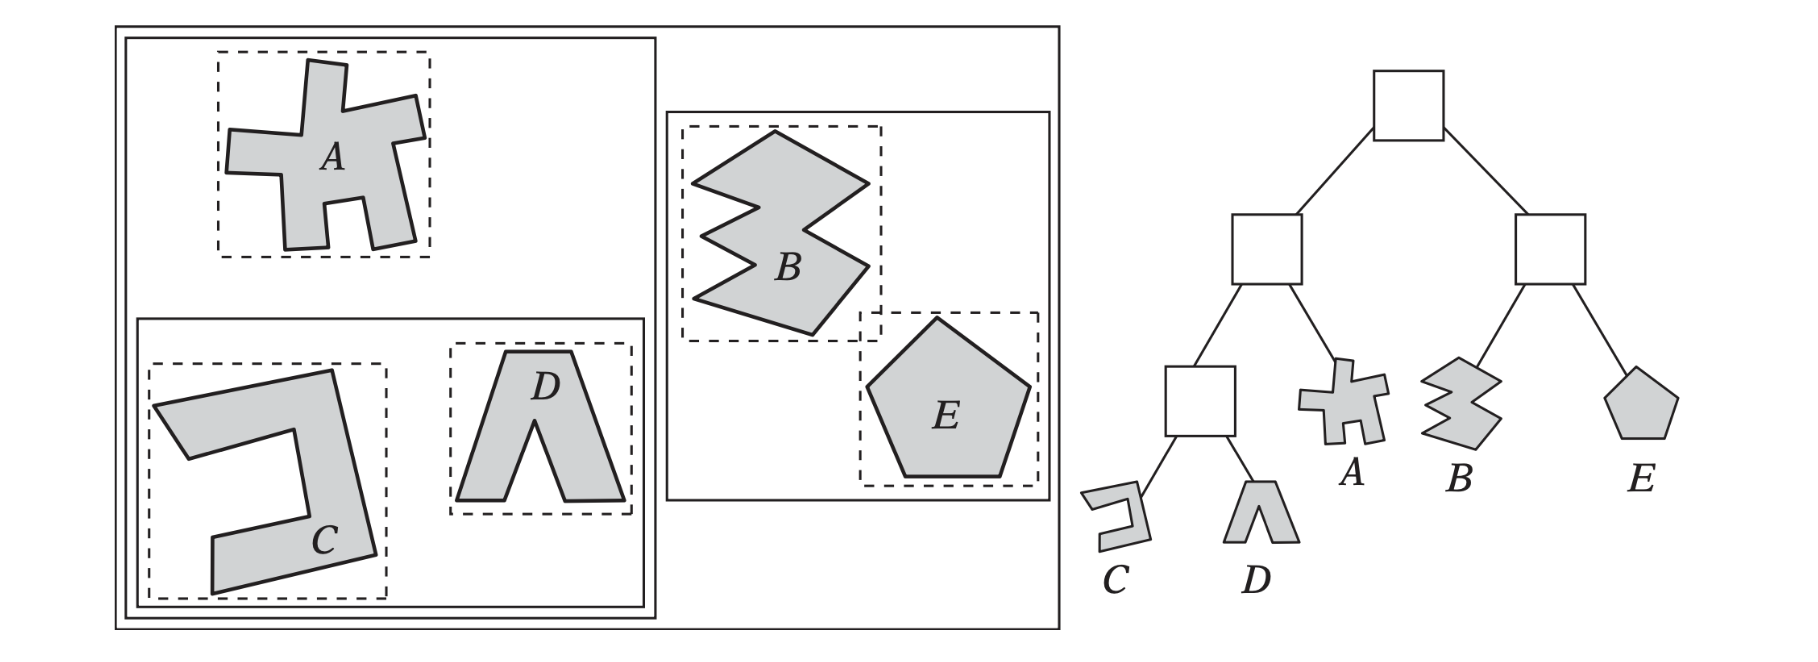
\includegraphics[width=.9\textwidth]{motion-planning/tree.png}
        \caption*{The associated configuration tree}
    \end{minipage}
\end{figure}

\subsection{Obstacles and collisions}

\newpage